\section{Introduction}
\label{sec:introduction}

% Outline: IoT for home entertainment
Internet-of-Things (IoT) technologies are being rapidly adopted in the consumer electronics market.
In addition to their use in traditional home automation systems, IoT technologies have also been applied to home entertainment. 
Especially with emerging virtual and augmented reality technologies, IoT offers the promise of new immersive and interactive experience for end-users.

Many IoT frameworks and ecosystems have been proposed to facilitate the development of more sophisticated applications.
They typically provide a similar set of framework-level services, including user and device authentication and authorization, device and service discovery, device management, publish-subscribe messaging, and remote access.
Fig.~\ref{fig:service-arch} shows a common hierarchical architecture of IoT services, where ``named entities'' refer to users, devices, and applications that require trust management and utilize rendezvous services to get organized into a coherent home IoT system.

\begin{figure}[!t]
\centering
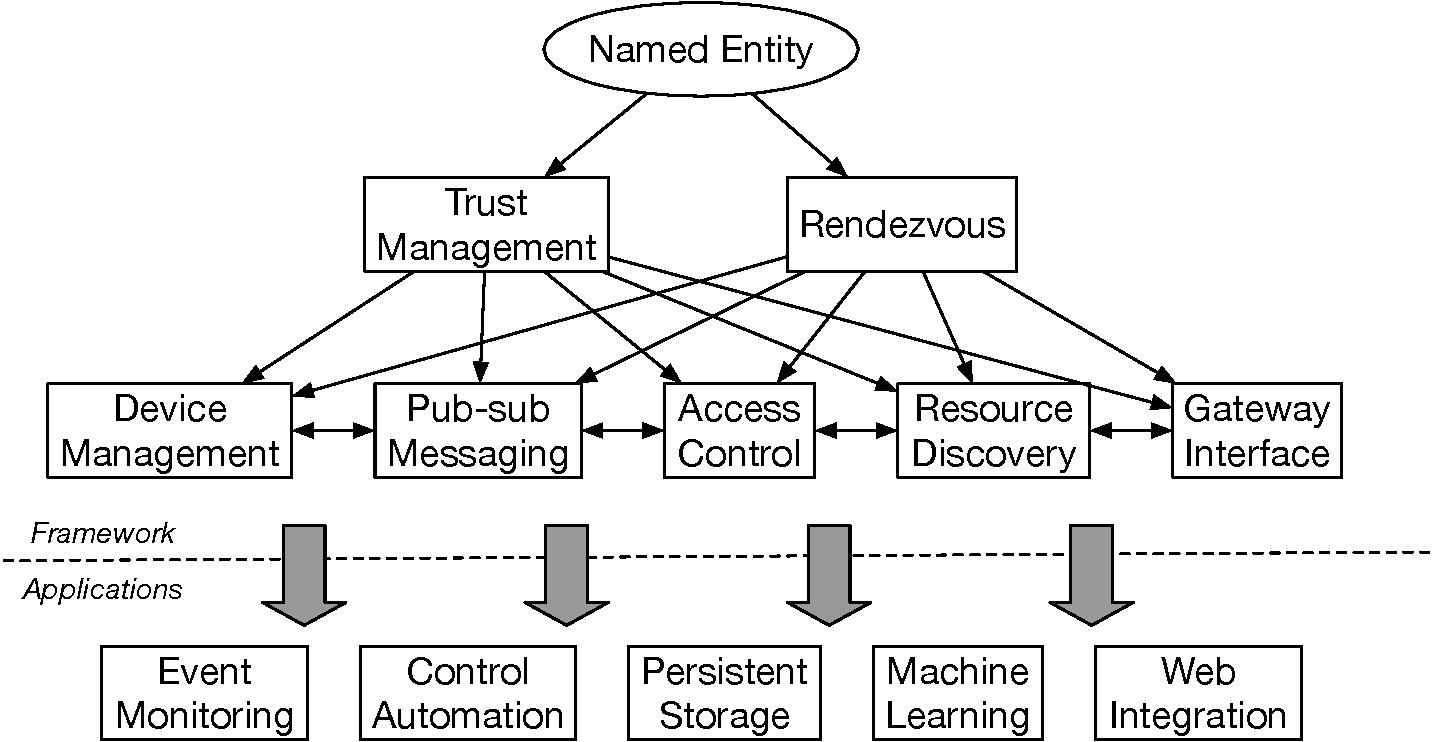
\includegraphics[width=0.95\columnwidth]{service-arch.pdf}
\caption{Hierarchical architecture of IoT services.}
\label{fig:service-arch}
\end{figure}

% Outline: introducing Flow
Flow application, a prototype home entertainment experience, takes an NDN approach~\cite{ccn-van,ndn}, and builds on our previous work in~\cite{ndn-iot} to achieve foundational functions of \emph{trust management} and \emph{rendezvous}.
While in the authors' IoTDI 2017 paper Flow application is used to illustrate the high-level concepts, this report focuses on an expanded description of lower-level details in the implementation of Flow and its underlying libraries.\footnote{Background study, key design insights, and conceptual evaluations are better covered in the IoTDI paper.}

% Outline: the rest of the paper
The rest of the report is structured as follows. 
In Section~\ref{sec:flow-overview}, we first give an overview of Flow application.
In Sections~\ref{sec:design} and~\ref{sec:implementation}, we present the design and implementation details of Flow, and finally conclude with Section\ref{sec:conclusion}.
% We then discuss a few practical application scenarios in Section~\ref{sec:scenarios}, and finally conclude with Section\ref{sec:conclusion}.